\section{Resultados} \label{sec:resultados}

A presente seção apresenta os resultados empíricos coletados a partir
dos algoritmos para fins de comparação entre seus tempos de execução
com base no tamanho de suas entradas, neste caso sendo o número de
vértices do grafo avaliado, resumidos na Tabela \ref{tab:dados_brutos}.

\begin{table}[hbtp]
  \centering
  \caption{Tempos médios de execução em milissegundos para grafos de
  tamanho $n$.}
  \label{tab:dados_brutos}
  \begin{tabular}{ccc}
    \toprule
    Tamanho da Entrada ($n$) & Dijkstra (ms) & Bellman-Ford (ms) \\
    \midrule
    100 & 0.5 & 1.2 \\
    200 & 2.1 & 5.8 \\
    300 & 4.8 & 15.2 \\
    \bottomrule
  \end{tabular}
\end{table}

Para melhor compreensão comparativa, os dados apresentados foram
plotados na Figura \ref{fig:grafico_tempos}, demonstrando visualmente
o distanciamento entre as curvas de tempo de execução à medida que o
tamanho da entrada aumenta.

\begin{figure}[hbtp]
  \centering
  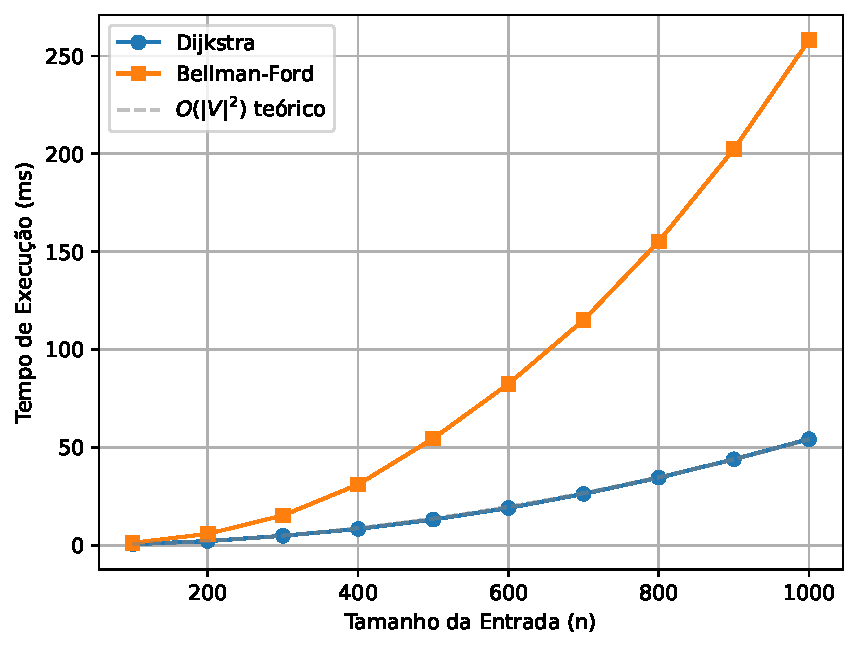
\includegraphics[width=0.8\textwidth]{grafico_tempos.pdf}
  \caption{Comparação do tempo de execução entre Dijkstra e Bellman-Ford.}
  \label{fig:grafico_tempos}
\end{figure}

\begin{figure}[hbtp]
  \centering
  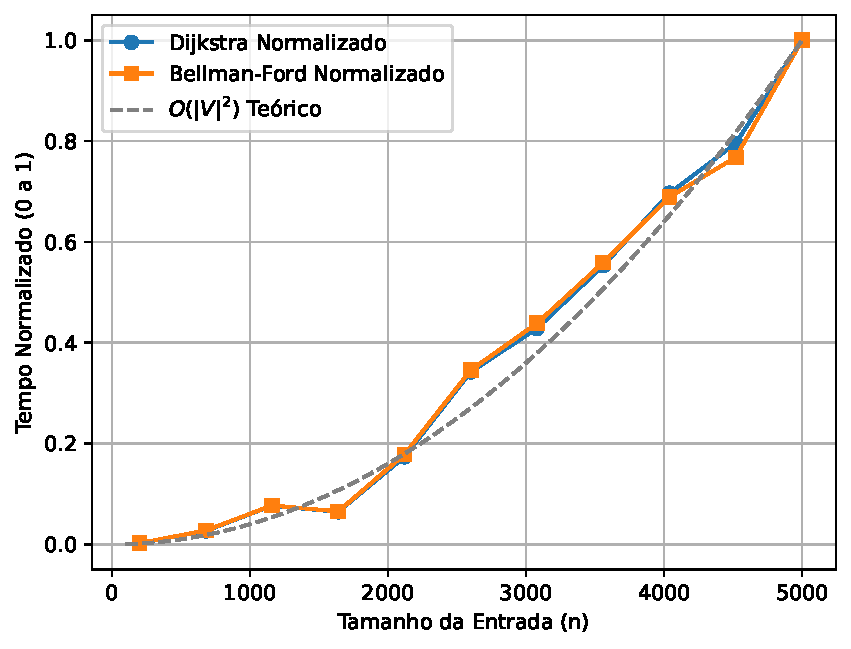
\includegraphics[width=0.8\textwidth]{grafico_normalizado.pdf}
  \caption{Comparação do tempo de execução normalizado entre Dijkstra
  e Bellman-Ford.}
  \label{fig:grafico_normalizado}
\end{figure}

A partir da leitura da Figura \ref{fig:grafico_tempos}, observa-se
que ao definir o eixo x como o tamanho de entrada e o eixo y como o
tempo de execução, [TODO: DESCREVER COMPORTAMENTO COM DADOS FINAIS].

Por outro lado, ao analisar o eixo x como tamanho de entrada e o eixo
y como o tempo de execução normalizado de 0 a 1, a Figura
\ref{fig:grafico_normalizado}, nota-se que as curvas dos algoritmos
alinham-se de maneira mais próxima a curva teórica de $O(|V|^2)$, sem
apresentar desvios significativos. A normalização, realizada por meio
da divisão da série de dados pelo valor máximo da curva, evidencia
que o perfil de crescimento de ambos os algoritmos reflete a mesma
complexidade polinomial.

\section{Discussão}

Sob a ótica dos resultados coletados, observa-se uma eficiência
notavelmente superior do algoritmo de Dijkstra em comparação ao
algoritmo de Bellman-Ford no que diz respeito à busca de caminhos em
roteamento intra-domínio. Os dados empíricos apresentados na Seção
\ref{sec:resultados} corroboram a análise teórica de
\cite{thippeswamy}, fortalecendo a premissa de que, embora ambos
resolvam o problema de busca do caminho mais curto a partir de uma
única origem, o algoritmo de Dijkstra desempenha este papel com menor
custo computacional. Portanto, para quantidades significantes de
arestas, há uma substancial vantagem ao utilizar a busca de menor
caminho por meio de Dijkstra.

Isto ocorre pois o algoritmo de Dijkstra se baseia em uma abordagem
gulosa, ou seja, a cada passo, é realizada uma escolha localmente
ótima, subsequentemente não reconsiderando escolhas passadas. Para
tal, o algoritmo seleciona o nó de peso mínimo que ainda não foi
processado para realizar o relaxamento das arestas. Isto torna o
algoritmo mais performático caso haja premissas estruturais baseadas
na existência exclusiva de pesos positivos. Dessa forma, sua
complexidade reflete a abordagem, configurando-se como
$O(|V|^2 + |E|)$, simplificada para $O(|V|^2)$.

Em contrapartida, o algoritmo de Bellman-Ford não adota uma
estratégia gulosa. Em vez disso, ele executa um processo exaustivo de
relaxamento de todas as arestas por exatas $|V| - 1$ vezes. Essa
repetição garante a correta propagação das distâncias mínimas por
todo o grafo e confere ao algoritmo a capacidade de processar arestas
com pesos negativos. No entanto, o custo computacional dessa
flexibilidade reflete-se em sua complexidade teórica de
$O(|V| \times |E|)$, o que acarreta um aumento drástico no
tempo de execução, especialmente à medida que o grafo se torna mais
denso, com um maior $|E|$.

Vale destacar que, para grafos de tamanho pequeno, o tempo de
execução de ambos os algoritmos é virtualmente idêntico, como
observado na Figura \ref{fig:grafico_tempos}. Com um tamanho de
entrada $n$ suficientemente pequeno, o tempo de alocação inicial das
estruturas e as constantes ocultas da notação dominam o tempo total,
atenuando a diferença entre o crescimento de $|V|^2$ e $|V| \times
|E|$. Diante dos resultados, o comportamento assintótico torna-se
substancial a partir de [TODO: qual tamanho de entrada define o
limiar de diferença], demonstrando o crescimento abrupto do algoritmo
de Bellman-Ford.

\section{Conclusão}

A análise empírica realizada neste trabalho confirma a superioridade
em eficiência do algoritmo de Dijkstra frente ao Bellman-Ford na
busca do caminho mais curto para roteamento intra-domínio. A
abordagem gulosa poupa processamento em comparação à varredura
exaustiva do Bellman-Ford, consolidando o Dijkstra como a escolha
ideal para grafos com pesos estritamente positivos por apresentar
tempos de execução consistentemente menores.

Ainda assim, o algoritmo de Bellman-Ford mantém sua relevância
fundamental em cenários de roteamento que admitem arestas de peso
negativo. Seu elevado custo computacional justifica-se pela
capacidade de encontrar caminhos em redes complexas de forma
confiável. É imperativo ressaltar, contudo, que caso existam ciclos
negativos alcançáveis a partir da origem, nenhum dos algoritmos é
capaz de computar o caminho mais curto, visto que o peso total
decresce infinitamente a cada travessia no ciclo.

Por fim, cabe destacar que os tempos absolutos aferidos nesta análise
são intrínsecos ao \textit{hardware} e ao sistema operacional
utilizados no experimento. Como direcionamento para trabalhos
futuros, sugere-se a execução de testes empíricos em grafos contendo
arestas negativas, a fim de demonstrar na prática a falha inerente do
algoritmo de Dijkstra e a resiliência do Bellman-Ford diante de tal cenário.
